\documentclass[11pt]{article}
\usepackage[utf8]{inputenc}
\usepackage{amsmath}
\usepackage{titlesec}
\usepackage{titling}
\usepackage{geometry}
\usepackage{media9}
\usepackage{graphicx}
\usepackage{hyperref}
\usepackage{fancyhdr}
\usepackage{wallpaper}
\usepackage{afterpage} 
\usepackage{pagecolor} 
\usepackage{multirow}
\usepackage{wrapfig}
\usepackage{lipsum} 
\usepackage{url}
\usepackage[toc,page]{appendix}
\usepackage{mdframed}
\usepackage{pgfgantt}
\usepackage{tabularx}


% Define colors
\usepackage{xcolor}
\definecolor{myblue}{RGB}{33, 66, 99}
\definecolor{mygray}{RGB}{169, 169, 169}
\definecolor{darkbluegrey}{RGB}{44, 62, 80} 

% Page styling
\pagestyle{fancy}
\fancyhf{}
\renewcommand{\headrulewidth}{0pt}
\renewcommand{\footrulewidth}{0pt}
\fancyfoot[C]{\thepage}
\renewcommand{\familydefault}{\sfdefault}

% Define a command for section headers
\titleformat{\section}
  {\color{myblue}\normalfont\Large\bfseries}
  {\color{myblue}\thesection}{1em}{}

% Define a command for subsection headers
\titleformat{\subsection}
  {\color{myblue}\normalfont\large\bfseries}
  {\color{myblue}\thesubsection}{1em}{}

% Adjust page margins
\geometry{a4paper, margin=1in}

% make references clickable
\hypersetup{
    colorlinks=true,
    linkcolor=blue,
    filecolor=magenta,      
    urlcolor=cyan,
}

\begin{document}

% Change the background color of the first page
\pagecolor{darkbluegrey}
\afterpage{\nopagecolor}

% Add a background image
\ThisCenterWallPaper{0.75}{./image/spike_brain.png}

\begin{titlepage}
  \vspace*{\stretch{1}}
  \begin{center}
    \textcolor{white}{\textbf{\Huge First Report}}\\ % changed text color to white
    \vspace{1cm}
    \textcolor{white}{\Large Sound Detection and Classification\\using Spiking Neural Networks} % changed text color to white
    \vspace{3cm}
  \end{center}
  \vspace*{\stretch{2}}
  \begin{center}
    \textcolor{white}{ % changed text color to white
      \textbf{COURREGE Téo}\\
      \textbf{GANDEEL Lo'aï}\\
      \vspace{1cm}
      \Large Date: \today}
  \end{center}
  \vspace*{\stretch{1}}
\end{titlepage}

\newpage

\tableofcontents

\pagebreak

\listoffigures

\pagebreak

\section{Introduction}

Our project addresses the challenge of applying spiking neural networks (SNNs) to audio classification in the field of spiking neural network research. This report provides an overview of our initial progress in this area. Our project specifically addresses the problem of audio classification within the broader context of SNNs.

Before delving into the details, we outline key aspects including preprocessing, data manipulation/augmentation, initial model implementations, and a look at preliminary results.

Using audio data primarily from the \href{https://research.google.com/audioset/}{Google AudioSet} database, our work involves preprocessing, which includes conversion of signals to image representations, feature extraction, and consideration of encoding schemes suitable for SNNs. Challenges related to data quality, context, and labeling complexity prompted the exploration of data augmentation strategies to improve model robustness.

In the following sections, we will elaborate on the organizational structure of our project, the technical environment utilized, a detailed account of the work accomplished, challenges faced and solutions implemented, concluding with a reflection on our achievements and future perspectives.




% Your content for the "Data" section goes here

\pagebreak

\section{The project}

\subsection{Description of the project - Spiking Neural Networks}

\subsubsection{Reminder of the Dow}

Inspired by the neural signaling patterns of the human brain, SNNs introduce a temporal element into artificial neural networks. This temporal characteristic positions SNNs as promising candidates for real-time processing and pattern recognition tasks.

A Spiking Neural Network is a variant of artificial neural networks designed to more accurately mimic biological neural networks. Unlike traditional artificial neural networks (ANNs) that work with continuously changing time values, SNNs operate with discrete events occurring at defined times. They take a set of spike values as input and produce a set of spike values as output.

The spiking behavior of a neuron in an SNN is modeled by a membrane potential equation. For instance, in a leaky integrate-and-fire (LIF) neuron model, the membrane potential equation is defined by a set of parameters including a time constant ($\tau$), resting potential ($u_{r1}$), reset potential ($u_{r2}$), synaptic weights ($w_j$), and a firing threshold ($u_th$). The output spike ($s$) is determined based on the membrane potential ($u$) and various conditions. This discrete event-based approach distinguishes SNNs from other types of neural networks.\cite{rething_comparison_ann_snn}

\begin{equation}
  \begin{cases}
    \tau \frac{d \: u(t)}{dt} = - [u(t) - u_{r_1}] + \sum_j w_j \sum_{t_j^k \in  S_i^{T_w}} K(t - t_j^k) \\
    \begin{cases}
      s(t) = 1 & u(t) = u_{r_2} \text{ if } u(t) \geq u_{th} \\
      s(t) = 0 & \text{otherwise}
    \end{cases}
  \end{cases}
  \label{eq:membrane_potential}
\end{equation}

%This equation describes the evolution of the membrane potential ($u$) over time, incorporating the influence of synaptic weights and input spike timings within a specified integration time window ($T_w$). The discrete output spike ($s$) is determined based on conditions related to the membrane potential, where a spike occurs if the potential surpasses both the firing threshold ($u_{th}$) and the reset potential ($u_{r_2}$).

This equation was firstly formulated as :
\begin{equation}
  \tau \frac{d \: u(t)}{dt} = - [u(t) - u_{r}] + RI
  \label{eq:lif_1}
\end{equation}

From a mathematical perspective, Equation (\ref{eq:lif_1}) represents a linear differential equation. Alternatively, an electrical engineer may recognize it as the equation of a leaky integrator or $RC$-circuit with parallel resistor ($R$) and capacitor ($C$). In the realm of neuroscience, this equation is termed the equation of a passive membrane. \cite{neuronal_dynamics}

\begin{figure}[h]
  \centering
  \begin{minipage}{0.45\textwidth}
    \centering
    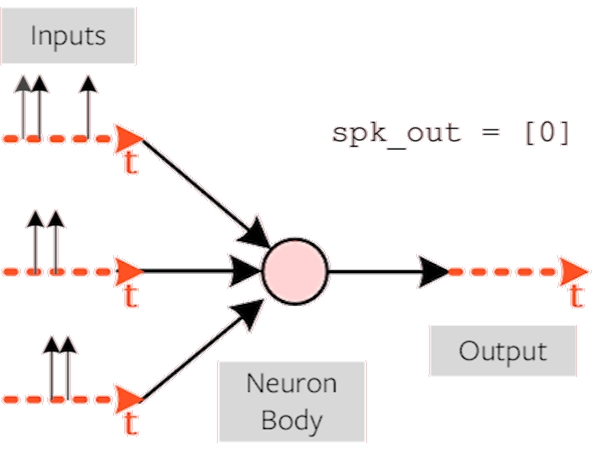
\includegraphics[width=1\textwidth]{image/def1.png}
    \caption{SNN input}
    \label{fig:def1}
  \end{minipage}\hfill
  \begin{minipage}{0.45\textwidth}
    \centering
    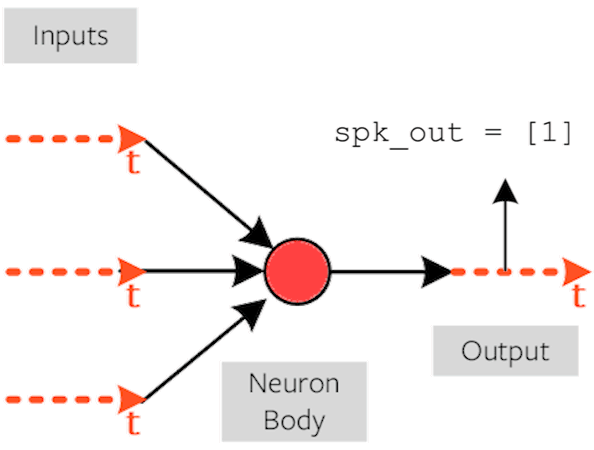
\includegraphics[width=1\textwidth]{image/def2.png}
    \caption{SNN output}
    \label{fig:def2}
  \end{minipage}
\end{figure}

\pagebreak

\subsubsection{Audio classification task}

Audio classification is a fundamental problem in the field of audio processing. It involves assigning a label to an audio clip based on its content. The audio classification task can be further divided into two subtasks: sound event detection (SED) and sound event classification (SEC). SED involves detecting the onset and offset times of sound events in an audio clip, while SEC involves assigning a label to each detected sound event.

In the context of audio classification, training an SNN involves working on image representations of audio data and encoding schemes suitable for SNNs.


\subsubsection{Objectives of the project}

The primary goal of our project is to exploit the temporal processing capabilities of SNNs for audio classification tasks. Specifically, we want to develop models capable of classifying (and possibly detecting) sound events from audio data.

Furthermore, knowing that SNNs consume less power than traditional Artificial Neural Networks (ANNs), but have lower overall accuracy, we want to perform a performance comparison of SNNs with ANNs.

The fullfillment of these objectives would allow us to determine the potential of SNNs for audio classification tasks and to identify the advantages and disadvantages of SNNs compared to other neural networks. Moreover, it is a great way for us to learn more about SNNs and audio classification.


\pagebreak

\section{Organizing the project}

\subsection{Main tasks}

During the last full time period, we worked on:

\begin{itemize}
  \item \textbf{A preprocessing pipeline} that allows us to dowload, format and segment the audio part of the Youtube videos composing the Google Audioset audio files into images.
        In order to be efficient, the pipeline needed to be parallelized.
        \subitem After downloading these, it became also necessary to perform some verification on the data, which includes checking the audio file properties (sample rate, number of channels, etc.) and the labels related to the audio files.
  \item \textbf{Finding some correct data augmentation techniques} that can be used to improve the performance of the SNNs.
  \item \textbf{Finding a way to encode the audio data into spikes} that can be used as input for the SNNs.
\end{itemize}

\begin{itemize}
  \item \textbf{Implementing the SNNs} that will be used for the audio classification task.
        \subitem Training the SNNs on the audio data.
  \item \textbf{Implementing the ANNs} that we would compare to the SNNs.
  \item \textbf{Comparing the performance of the SNNs and the ANNs} on the audio classification task.
\end{itemize}


\subsection{Planning and team organization}

\subsubsection{Previous work - full time period}

\begin{figure}[h]
  \centering
  \resizebox{0.85\textwidth}{!}{
    \begin{ganttchart}[
        hgrid,
        vgrid,
        x unit=1.0cm,
        y unit title=0.7cm,
        y unit chart=0.9cm,
        title label font=\footnotesize,
        group label font=\footnotesize,
        milestone label font=\footnotesize,
        bar label font=\footnotesize,
        bar label node/.append style={align=left, text width=3cm}
      ]{1}{12}

      \gantttitle{Days}{12} \\
      \gantttitlelist{1,...,12}{1} \\

      \ganttgroup{\textbf{Setup and Literature Review}}{1}{1} \\

      \ganttgroup{\textbf{Working on the data}}{2}{6} \\
      \ganttbar[bar label node/.append style={align=left},
        bar/.append style={fill=red}]{Download, Format and Segment}{2}{5} \\
      \ganttbar[bar label node/.append style={align=left},
        bar/.append style={fill=blue}]{Data transformation}{2}{6} \\
      \ganttgroup{\textbf{Verification and SnnToch}}{6}{10} \\
      \ganttbar[bar label node/.append style={align=left},
        bar/.append style={fill=red}]{Data Verification and debugging}{6}{9} \\
      \ganttbar[bar label node/.append style={align=left},
        bar/.append style={fill=blue}]{Handling SnnTorch}{7}{10} \\

      \ganttgroup{\textbf{First implementations}}{11}{12} \\
      \ganttbar[bar label node/.append style={align=left},
        bar/.append style={fill=red}]{Testing ANNs}{11}{12} \\
      \ganttbar[bar label node/.append style={align=left},
        bar/.append style={fill=blue}]{Develop Spike Encoding}{11}{12} \\

    \end{ganttchart}
  }% Add this line
  \caption{Planning of the full time period}
  \label{fig:ftp1}
\end{figure}

\begin{itemize}
  \item Téo : \textcolor{blue}{blue}
  \item Loaï : \textcolor{red}{red}
\end{itemize}

So far, we have been able to encode and decode the audio data into spikes.

%We were also able to train an ANN on the audio data and test it on the audio classification task. 

Since the first tasks we had to perform would not be connected until they were finished, we decided to work on them in parallel. This allowed us to be more efficient and, most importantly, to save time.

\subsection{Changes in the organization}

In the initial planning, there was no task related to the verification of the data nor to the debugging of part of the code. Each subpart of the preprocessing pipeline part takes a lot of time to be implemented and tested. We had to spend some time debugging the code and verifying the data.

%Handling the SnnTorch library also took more time than expected.

\pagebreak

\section{Technical environment}

\subsection{Computational tools}

We worked on our personal computers and we used the following computational tools:


\begin{figure}[h]
  \begin{center}
    \begin{tabularx}{\textwidth}{|X|X|}
      \hline
      \textbf{Softwares}  & \href{https://code.visualstudio.com/}{Visual Studio Code}     \\
                          & \href{https://jupyter.org/}{Jupyter Notebook}                 \\
                          & \href{https://git-scm.com/}{Git}                              \\
                          & \href{https://github.com/}{Github}                            \\
                          & \href{https://colab.research.google.com/}{Google Colab}       \\
                          & \href{https://www.anaconda.com/products/individual}{Anaconda} \\
                          & \href{https://www.overleaf.com/}{Overleaf}                    \\
      \hline
      \textbf{Programming languages}
                          & \href{https://www.python.org/}{Python}                        \\
                          & \href{https://www.latex-project.org/}{Latex}                  \\
      \hline
      \textbf{Libraries}  & \href{https://pytorch.org/}{Pytorch}                          \\
                          & \href{https://librosa.org/doc/latest/index.html}{Librosa}     \\
                          & \href{https://numpy.org/}{Numpy}                              \\
                          & \href{https://pandas.pydata.org/}{Pandas}                     \\
                          & \href{https://matplotlib.org/}{Matplotlib}                    \\
                          & \href{https://pysox.readthedocs.io/en/latest/}{sox}           \\
                          & \href{https://github.com/ytdl-org/youtube-dl}{Youtube-dl}     \\
      \hline
      \textbf{Frameworks} & \href{https://github.com/eriksoper/SnnTorch}{SnnTorch}        \\
      \hline
    \end{tabularx}
  \end{center}
  \caption{Computational tools}
\end{figure}

\href{https://github.com/LGPolytech/Project_S9}{(Our Github repository)}



\subsection{Documentation}

\subsection{Changing}

\pagebreak

\section{Work accomplished}

\subsection{Data}

Notes: In the section below, we decided not to include some code snippets because they were not very relevant to the report.

\subsubsection{The Audioset}

In order to use the Google Audioset dataset, we needed to download the audio files and their associated labels. This first resulted in a file containing the links to the audio files and a file containing the label(s) of the audio files.
Their structure is as follows:

\begin{figure}[h]
  \centering
  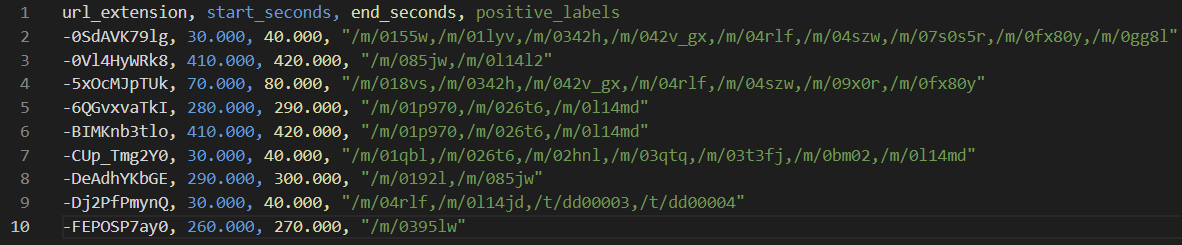
\includegraphics[width=\textwidth]{./image/structure_csv1.png}
  \caption{Structure and small content of the csv file containing the links to the audio files}
  \label{fig:structure_csv1}
\end{figure}

\subsubsection*{Filtering the data by labels}

The first column contains the links to the YouTube video, then the start and end time of the audio segment in the video, and finally the labels of the audio segment (there can be multiple labels for one audio segment).

Since we want to train our first model on small scenarios with only 3 classes \href{https://research.google.com/audioset/ontology/animal_1.html}{Animals}, \href{https://research.google.com/audioset/ontology/sounds_of_things_1.html}{Sound of things}, and \href{https://research.google.com/audioset/ontology/music_1.html}{Music}, we had to filter the data so that in all the rows that make up the csv file, there is at least one of the 3 classes we wanted to keep, but no repetition between the 3 classes.

Basically, we needed to iterate over the initial csv file to create 3 csv files, each containing only videos with one of the 3 classes we wanted to keep (see \texttt{reorder\_to\_categories.py}).

Also, there might be some repetitions between the labels associated with each audio segment, so we needed to remove those duplicates (see \texttt{reorder\_btw\_categories.py}).

(see our \href{https://github.com/LGPolytech/Project_S9}{GitHub repository}).

\subsubsection*{Downloading the audio files}

Once we had the csv files containing the links to the audio files, we needed to download them. To do this, we started using this \href{https://github.com/bakhtos/GoogleAudioSetScripts}{Github} repository as a base for our work. Since there were some problems using the \texttt{youtube-dl} library (that was changes to the \texttt{yt-dlp}), we had to modify the code to allow parallelization of the process (crucial for the efficiency of the pipeline if we don't want to wait for days to download the audio files).

We ended up with a code similar to the first one, but with some compatibility, performance and parallelization improvements (see \texttt{main\_dfs.py}).

\subsubsection*{Checking the data}

Once we had downloaded the audio files, we had to check that all the registered ones were not missing some information, corrupted or of duration less than 10 seconds (see \texttt{valid\_with\_labels}). This part ended-up being a source of problems as it consisted in a test and debug part.

\pagebreak


\subsection{Study of SNNs}

\subsubsection{Neurons model}
1. Leaky Integrate-and-Fire (LIF) Neuron:

The LIF neuron model is a simple but commonly used model in spiking neural networks.


Equation:

\begin{align*}
    \tau_m \frac{du}{dt} = -[u(t) - u_{\text{rest}}] + RI(t)
\end{align*}



2. Hodgkin-Huxley (HH) Neuron:

The Hodgkin-Huxley model is a more complex and biophysically detailed model.

Equations:

\begin{align*}
C_m \frac{dV}{dt} &= -I_{\text{Na}} - I_{\text{K}} - I_{\text{L}} + I_{\text{ext}} \\
I_{\text{Na}} &= g_{\text{Na}} m^3 h (V - E_{\text{Na}}) \\
I_{\text{K}} &= g_{\text{K}} n^4 (V - E_{\text{K}}) \\
I_{\text{L}} &= g_{\text{L}} (V - E_{\text{L}}) \\
\frac{dm}{dt} &= \alpha_m (1 - m) - \beta_m m \\
\frac{dh}{dt} &= \alpha_h (1 - h) - \beta_h h \\
\frac{dn}{dt} &= \alpha_n (1 - n) - \beta_n n \\
\end{align*}


\begin{flushleft}
\begin{description}
    \item[$C_m$:] Membrane capacitance
    \item[$V$:] Membrane potential
    \item[$I_{\text{*}}$:] Sodium, Potassium, leakage, and external current
    \item[$g_{\text{*}}$:] Maximum sodium, potassium, and leakage conductance
    \item[$E_{\text{*}}$:] Nernst potential for sodium, potassium, and leakage (the equilibrium potential)
    \item[$m, h, n$:] Gating variables that represent the fraction of channels in the open state for sodium, potassium, and leakage channels, respectively
    \item[$\alpha_m, \beta_m, \alpha_h, \beta_h, \alpha_n, \beta_n$:] Voltage-dependent rate constants governing the kinetics of the opening and closing of ion channels
\end{description}
\end{flushleft}



3. Izhikevich Neuron:

The Izhikevich neuron model is a two-dimensional model designed to capture a wide range of spiking behaviors.

Equations:

\begin{align*}
\frac{dv}{dt} &= 0.04v^2 + 5v + 140 - u + I_{\text{syn}} \\
\frac{du}{dt} &= a(bv - u)
\end{align*}


Parameters:

    $v$: Membrane potential
    
    $u$: Membrane recovery variable
    
    $a,ba,b$: Parameters determining the neuron's behavior
    
    $I_{\text{syn}}$​: Synaptic current


Although it is not the one which represents reality the most, LIF model is the best compromise if we take into account computation complexity.

\begin{figure}[h]
  \centering
  \begin{minipage}{0.9\textwidth}
    \centering
    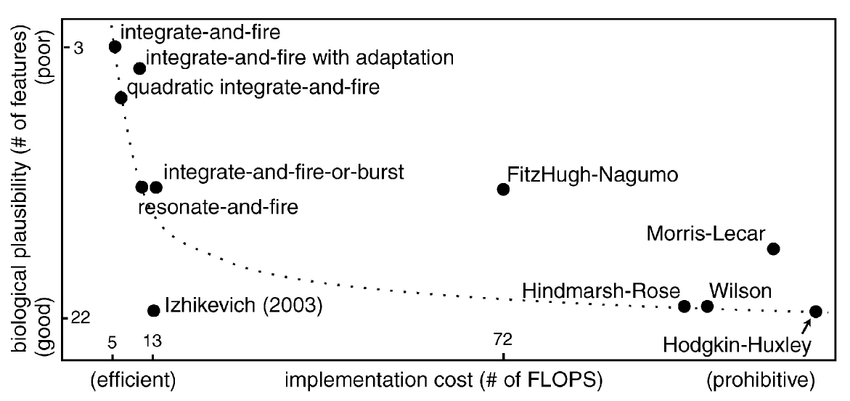
\includegraphics[width=1\textwidth]{"image/comparison_neuron.png"}
    \caption{Comparison of different neuron model's complexity and biological similarity}
    \label{fig:neuron_comparison}
  \end{minipage}\hfill
\end{figure}



\subsubsection{Spike encoding}

The encoding in SNNs refers to how information is represented and transmitted through the spikes of the SNN. In our study, we focus primarily on two of them:

    Rate Encoding:
    In rate encoding, information is represented by the firing rate of neurons. The more spikes a neuron produces within a given time window, the higher the firing rate, and the stronger the encoded information.


    Latency Encoding:
    Temporal encoding focuses on the precise timing of spikes. The timing information of individual spikes is crucial for representing the input data.
    The exact timing of spikes can convey additional information, and the temporal patterns of spikes are used to encode features or events in the input signal.




\subsection{Spectrograms, Mel spectrograms, MFCC}


    - Spectrograms

Spectrograms are essential graphic tools in audio analysis. They offer a visual representation of the frequency spectrum of a sound signal as a function of time, providing detailed information on the frequency composition and temporal dynamics of an audio signal. This report explores the use of spectrograms in various contexts and highlights their importance in the analysis and understanding of audio signals.

A spectrogram is generated by applying a short-time Fourier transform (STFT) to an audio signal. This technique divides the signal into small time windows, then applies a Fourier transform to each window to obtain the frequency distribution at that particular moment. The results of these transformations are then represented graphically, using colors to indicate the intensity of frequencies at different periods.



\begin{figure}[h]
    \begin{equation}
      X_k = \sum_{n=0}^{N-1} x_n e^{-i 2 \pi k n / N}
      \label{eq:fourier_transform}
    \end{equation}
    \caption{Discrete Fourier Transform}
\end{figure}

Spectrograms enable in-depth analysis of the temporal characteristics of audio signals. Events such as transients, attacks and decays can be clearly identified, which is essential for understanding dynamic variations in music, speech and other forms of sound.

By examining the color and intensity of areas in a spectrogram, it's easy to identify the dominant frequencies present in an audio signal. This is particularly useful for detecting anomalies, characterizing musical instruments and separating sound sources.

Spectrograms are widely used in fields such as professional audio, music and linguistics. In particular, we are interested in Mel spectrograms, as well as MFCCs as input data for our neural networks.


\begin{figure}[h]
  \centering
  \begin{minipage}{0.9\textwidth}
    \centering
    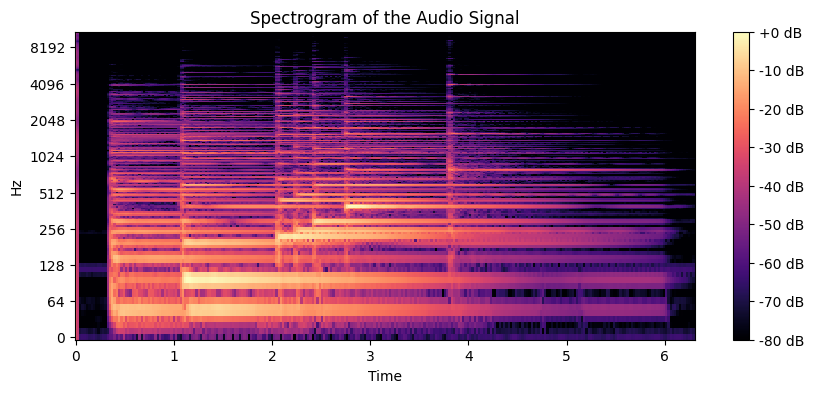
\includegraphics[width=1\textwidth]{"image/Spectrogram_piano.png"}
    \caption{Spectrogram of a slowly ascending piano arpeggio, we can notice the new notes with higher frequencies appearing over time, where the image is brighter}
    \label{fig:Spectrogram_piano}
  \end{minipage}\hfill
\end{figure}


    - Mel Spectrograms
    
While spectrograms offer a detailed view of the frequency spectrum of an audio signal, a significant evolution in audio analysis occurred with the introduction of Mel Spectrograms.

These represent an adaptation of traditional spectrograms, using a frequency scale based on the Mel scale, which is more in line with human auditory perception. This transition to Mel Spectrograms has broadened the possibilities of analysis, offering a more faithful representation of the auditory characteristics perceived by the human ear. Let's take a closer look at this innovation and its impact on modern audio analysis.

While spectrograms offer a detailed view of the frequency spectrum of an audio signal, a significant evolution in audio analysis occurred with the introduction of Mel Spectrograms. These represent an adaptation of traditional spectrograms, using a frequency scale based on the Mel scale, which is more in line with human auditory perception.

\begin{figure}[h]
  \centering
  \begin{minipage}{0.9\textwidth}
    \centering
    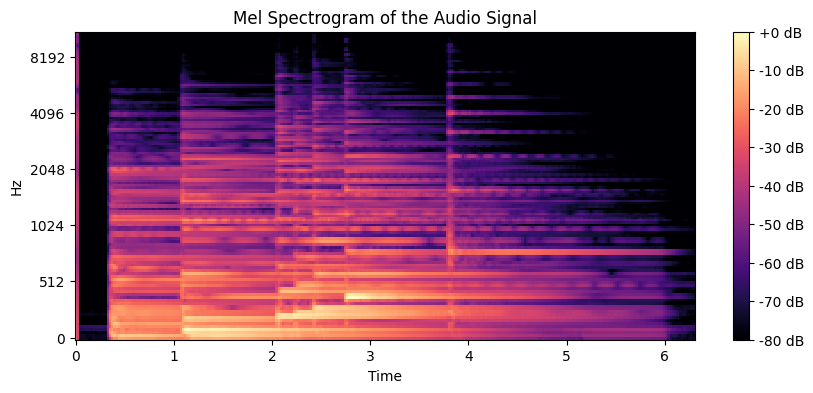
\includegraphics[width=1\textwidth]{"image/Mel_spectrogram_piano.png"}
    \caption{Mel Spectrogram, one of the main differences is that the bands corresponding to a note of the arpeggio are closer than in the spectrogram, which represents better the human auditory system}
    \label{fig:Mel_spectrogram_piano}
  \end{minipage}\hfill
\end{figure}


    - MFCC

MFCCs are derived directly from Mel Spectrograms and are calculated by applying a discrete cosine transform to the log-power of Mel Spectrograms. This approach captures information specific to human auditory characteristics while reducing data redundancy.MFCCs thus encapsulate frequency variations over time in a compact way, creating a set of cepstral coefficients that are widely used for automatic speech recognition and other audio signal processing tasks.

Two of the main advantages of MFCCs are compactness and information discrimination. MFCCs condense information while retaining the signal's distinctive characteristics. Compact representation facilitates the storage, transmission and processing of large amounts of data
By focusing on perceptual features rather than raw frequency, MFCCs are less sensitive to pitch variations, which improves the robustness of sound recognition.
The calculation of MFCCs involves several steps, including Mel scale transformation, calculation of the logarithm of spectral powers, discrete cosine transformation and selection of relevant coefficients.



To summarize, in order to obtain an MFCC from an audio signal:

- Take the Fourier transform (STFT) of the signal.

- Map the powers of the resulting spectrum onto the mel scale, multiplying it by overlapping window functions (triangular or cosinusoidal).

- Take the logarithm of the amplitudes at each mel frequency.

- Take the discrete cosine transform (DCT) of the list of logarithmic powers of the mel frequencies, as if it were a signal. The MFCCs are the amplitudes of the resulting spectrum.


\begin{figure}[h]
  \centering
  \begin{minipage}{0.75\textwidth}
    \centering
    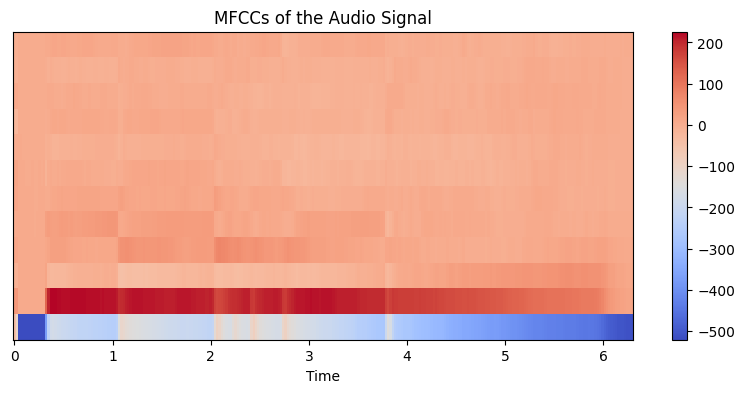
\includegraphics[width=1\textwidth]{"image/MFCC_piano.png"}
    \caption{MFCC}
    \label{fig:MFCC_piano}
  \end{minipage}\hfill
\end{figure}



\begin{equation}
  X_k = \sum_{n=0}^{N-1} x_n \cos \left[ \frac{\pi}{N} \left( n + \frac{1}{2} \right) k \right]
  \label{eq:dct}
\end{equation}



\subsection{Signal reconstruction}

To compare most used encoding methods, we used an SNN model to encode and then decode MFCCs extracted from an audio signal. The two most used encoding approaches were compared: frequency encoding and latency encoding.

RESULTS: Reconstruction quality

The results showed that latency encoding (when normalized and linearized and with a sufficient number of time steps) led to a better reconstruction quality of the audio signal than frequency encoding, which was much more subject to small errors that propagate during reconstruction, the errors being due to the probability of emitting a pulse for each time step, which does not perfectly represent the pixel intensity. This improvement can be explained by the ability of latency encoding to capture fine temporal variations in the signal. However, due to the loss of information during signal transformation in MFCC, and more specifically during DCT, no reconstruction reaches the quality of the original signal.

Moreover, with latency encoding, one pulse carries much more information, which can lead to less robustness in the face of noise, which can be very present in our dataset. We will therefore try to compare the two approaches in our SNN.

\begin{figure}[h]
  \centering
  \begin{minipage}{0.45\textwidth}
    \centering
    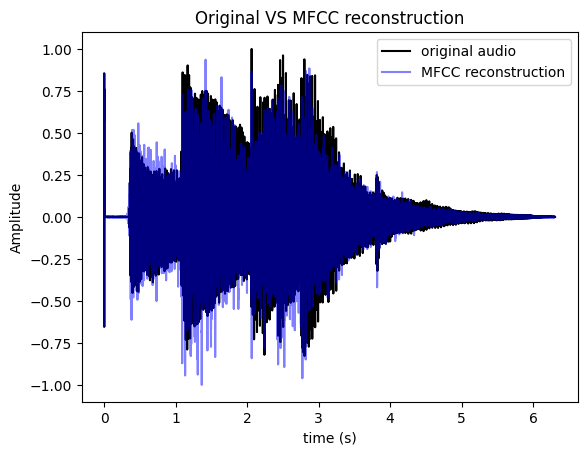
\includegraphics[width=1\textwidth]{"image/Original VS MFCC reconstruction.png"}
    \caption{Original VS MFCC reconstruction}
    \label{fig:OVSM}
  \end{minipage}\hfill
\end{figure}


\begin{figure}[h]
  \centering
  \begin{minipage}{0.45\textwidth}
    \centering
    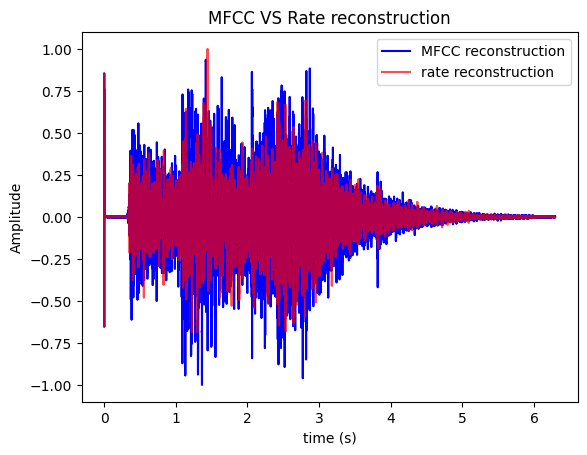
\includegraphics[width=1\textwidth]{"image/MFCC VS Rate reconstruction.png"}
    \caption{MFCC VS Rate reconstruction}
    \label{fig:MVSR}
  \end{minipage}\hfill
  \begin{minipage}{0.45\textwidth}
    \centering
    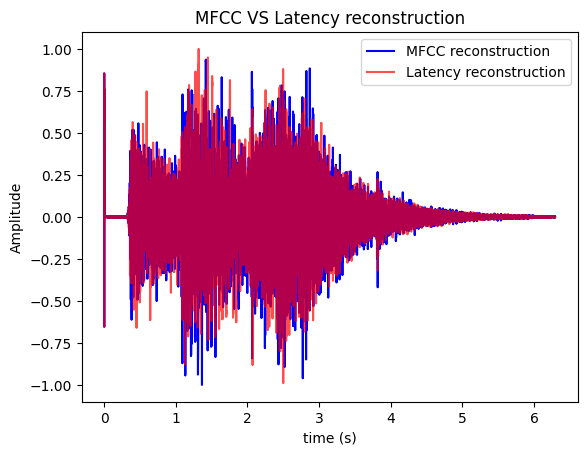
\includegraphics[width=1\textwidth]{"image/MFCC VS Latency reconstruction.png"}
    \caption{MFCC VS Latency reconstruction}
    \label{fig:MVSL}
  \end{minipage}
\end{figure}


\pagebreak


\section{Difficultés rencontrées}

%•	Description des difficultés principales rencontrées durant le projet et des solutions mises en place (si cela était possible).
%•	Les commentaires lors de la première soutenance ont-ils été utiles ?


For the reconstruction of the audio, the data needed to be properly normalized to create the MFCC and then denormalized to extract good audio. We used the MinMaxScaler of sklearn fitted on the data to achieve our results.



\pagebreak

\section{Conclusion et perspectives}

•	Mettre en valeur votre travail et les domaines où vous avez progressé.
•	Souligner en quoi la formation suivie à Polytech Nice Sophia (ou ailleurs) vous a aidé.
•	Que comptez-vous faire dans les prochaines semaines ?

\pagebreak

\subsection{Audio samples}
\begin{figure}[h]
  \centering
  \resizebox{0.8\textwidth}{!}{
    \begin{minipage}{.45\textwidth}
      \centering
      \includemedia[
        width=\textwidth,
        addresource=audio/piano_original.wav,
        flashvars={
            source=audio/piano_original.wav
            &autoPlay=false
            &hideBar=false
          },
      ]{\fbox{Play}}{APlayer.swf}
      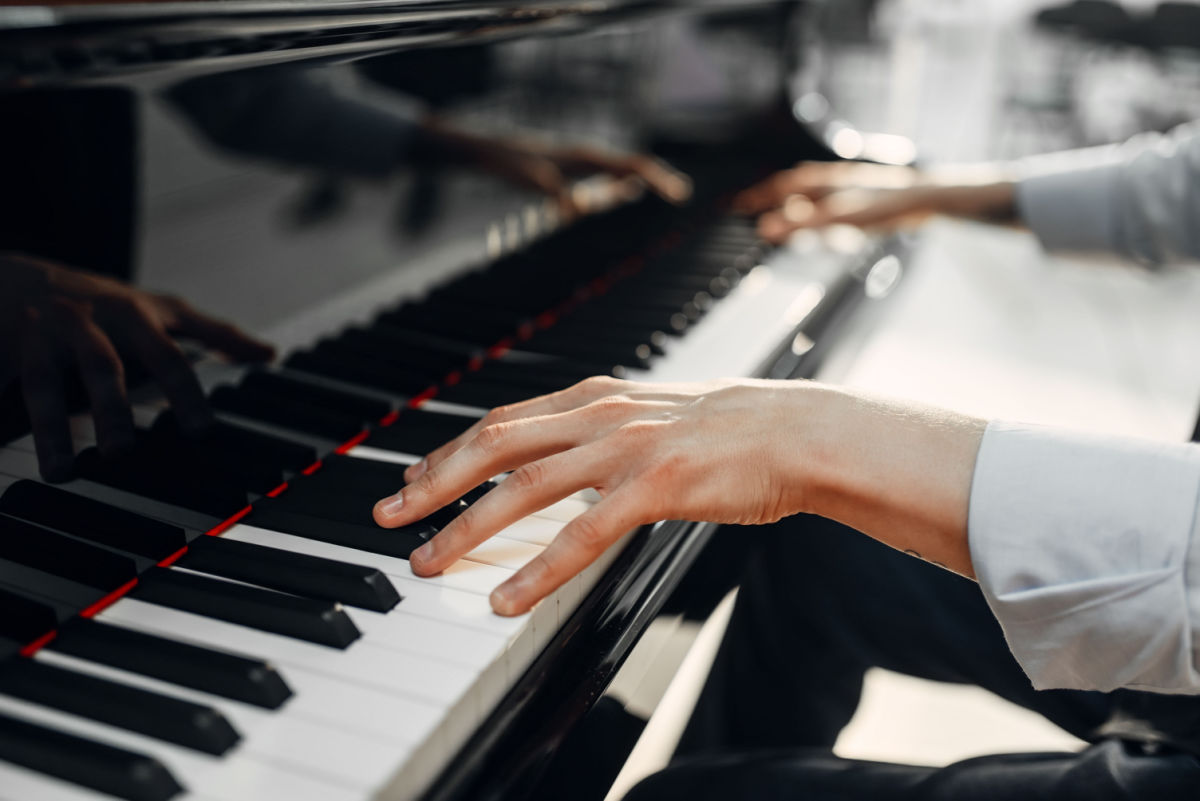
\includegraphics[width=\textwidth]{image/piano.png}
      \caption{Original Audio}
    \end{minipage}
    \begin{minipage}{.45\textwidth}
      \centering
      \includemedia[
        width=\textwidth,
        addresource=audio/piano_mfcc_reconstruction.wav,
        flashvars={
            source=audio/piano_mfcc_reconstruction.wav
            &autoPlay=false
            &hideBar=false
          },
      ]{\fbox{Play}}{APlayer.swf}
      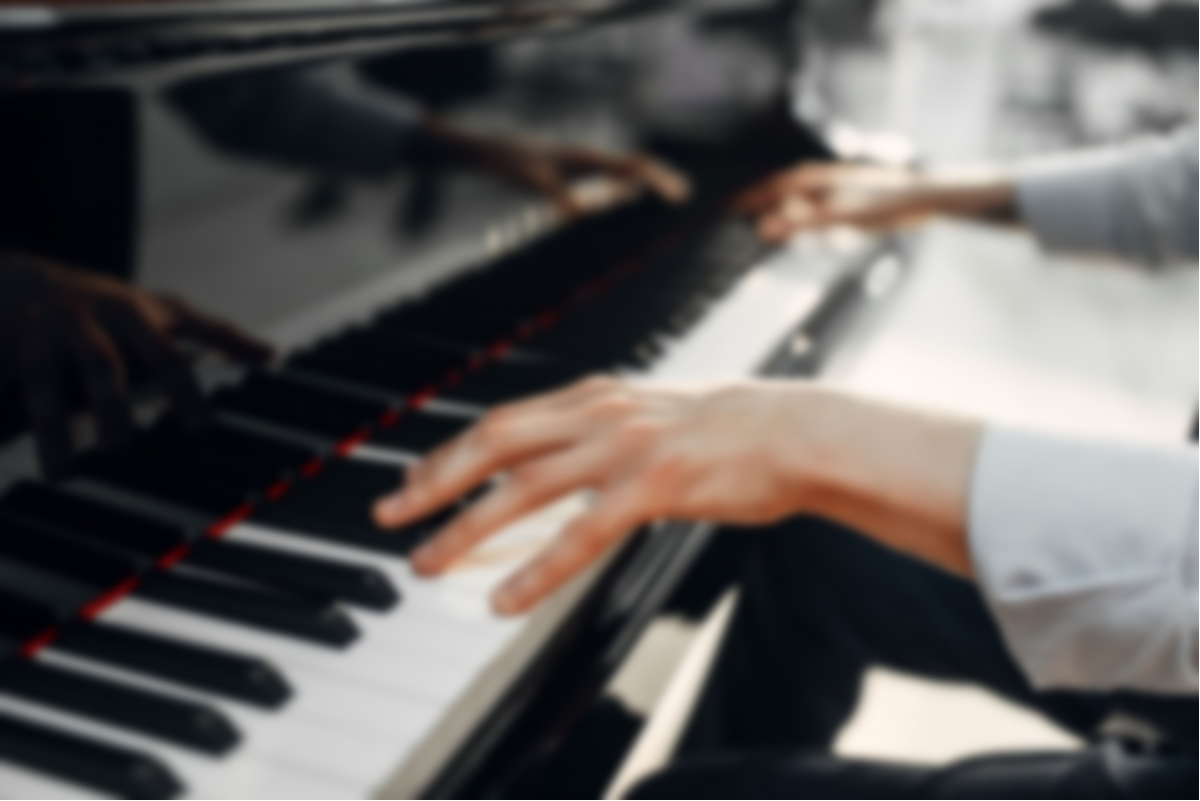
\includegraphics[width=\textwidth]{image/piano_blur1.png}
      \caption{MFCC Reconstruction}
    \end{minipage}
  }
\end{figure}

\begin{figure}[h]
  \centering
  \resizebox{0.8\textwidth}{!}{
    \begin{minipage}{.45\textwidth}
      \centering
      \includemedia[
        width=\textwidth,
        addresource=audio/piano_latency_reconstruction.wav,
        flashvars={
            source=audio/piano_latency_reconstruction.wav
            &autoPlay=false
            &hideBar=false
          },
      ]{\fbox{Play}}{APlayer.swf}
      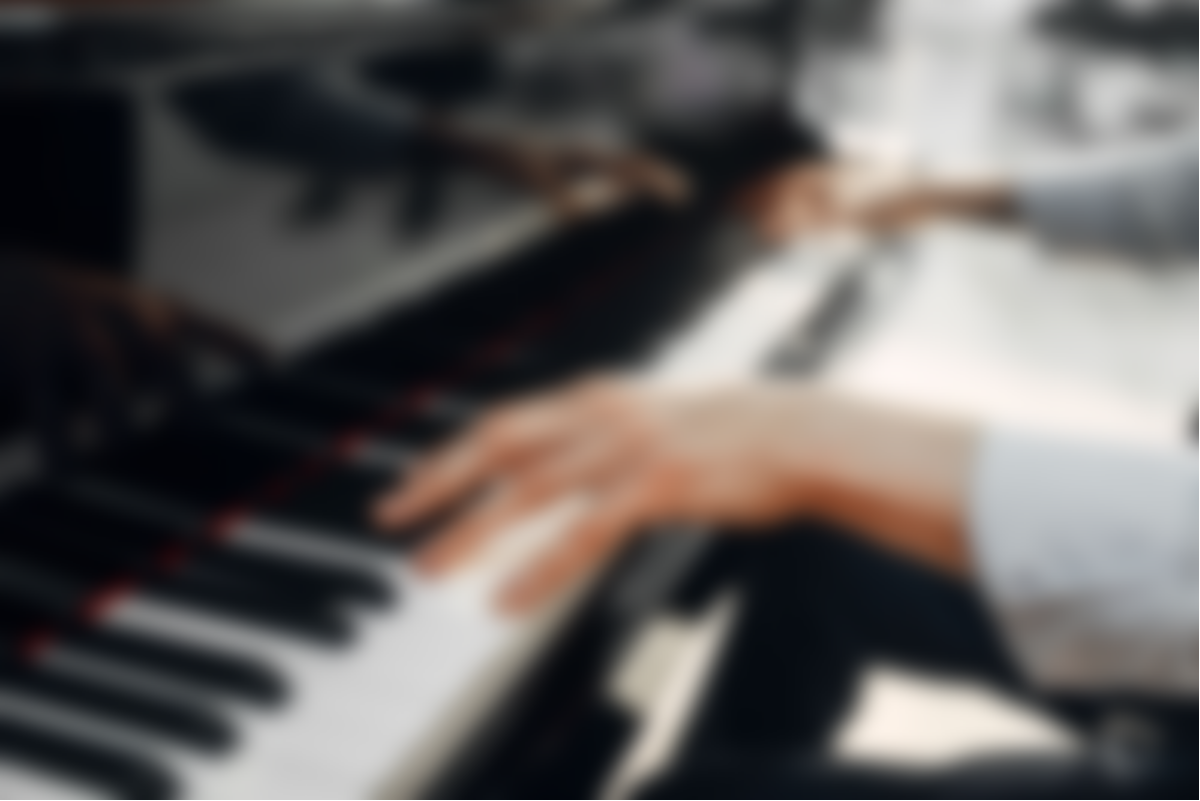
\includegraphics[width=\textwidth]{image/piano_blur2.png}
      \caption{Latency Reconstruction}
    \end{minipage}
    \begin{minipage}{.45\textwidth}
      \centering
      \includemedia[
        width=\textwidth,
        addresource=audio/piano_rate_reconstruction.wav,
        flashvars={
            source=audio/piano_rate_reconstruction.wav
            &autoPlay=false
            &hideBar=false
          },
      ]{\fbox{Play}}{APlayer.swf}
      
\includegraphics[width=\textwidth]{image/piano_blur3.png}
      \caption{Rate Reconstruction}
    \end{minipage}
  }
\end{figure}


\pagebreak

% Bibliography
\bibliographystyle{siam}
\bibliography{ref}

\end{document}